\documentclass[mathserif,9pt]{beamer}
\usepackage{indentfirst,mathrsfs}
\usepackage{amssymb}
\usepackage{pifont}
\usepackage{amsfonts}
\usepackage{booktabs}
\usepackage{color} 
\usepackage{bbm}
\usepackage{graphicx} 
\usepackage{indentfirst,mathrsfs}
\setbeamertemplate{footline}[frame number]

\usetheme{Darmstadt}

\usepackage{times}
\usefonttheme{structurebold}

\usepackage[english]{babel}
\usepackage{pgf,pgfarrows,pgfnodes,pgfautomata,pgfheaps}
\usepackage{amsmath,amssymb,mathrsfs}
\usepackage[latin1]{inputenc}
\usepackage{color}
\beamertemplatetextbibitems
\setbeamercovered{dynamic}



\definecolor{rgb0}{rgb}{1.0,0.5,0.5}
\definecolor{rgb1}{rgb}{0.0,0.5,0.5}
\definecolor{rgb2}{rgb}{0.8,0.6,0.6}
\definecolor{rgb3}{rgb}{0.1,0.7,0.6}

\newtheorem{property}{Property}
\newcommand{\GF}{{\bf GF}}



\pgfdeclaremask{tu}{beamer-tu-logo-mask}
\pgfdeclaremask{computer}{beamer-computer-mask}
\pgfdeclareimage[interpolate=true,mask=computer,height=2cm]{computerimage}{beamer-computer}
\pgfdeclareimage[interpolate=true,mask=computer,height=2cm]{computerworkingimage}{beamer-computerred}
\pgfdeclareimage[mask=tu,height=.5cm]{logo}{beamer-tu-logo}

\logo{\pgfuseimage{logo}}
\title{Cube attack and SHA-3 }

\author{Liu zhang}
\institute{Department of Computer Science, Shdantou University}
\colorlet{redshaded}{red!25!bg} \colorlet{shaded}{black!25!bg}
\colorlet{shadedshaded}{black!10!bg}
\colorlet{blackshaded}{black!40!bg}

\colorlet{darkred}{red!80!black} \colorlet{darkblue}{blue!80!black}
\colorlet{darkgreen}{green!80!black}

\def\radius{0.96cm}
\def\innerradius{0.85cm}

\def\softness{0.4}
\definecolor{softred}{rgb}{1,\softness,\softness}
\definecolor{softgreen}{rgb}{\softness,1,\softness}
\definecolor{softblue}{rgb}{\softness,\softness,1}

\definecolor{softrg}{rgb}{1,1,\softness}
\definecolor{softrb}{rgb}{1,\softness,1}
\definecolor{softgb}{rgb}{\softness,1,1}

\newcommand{\Bandshaded}[2]{
  \color{shadedshaded}
  \pgfmoveto{\pgfxy(-0.5,0)}
  \pgflineto{\pgfxy(-0.6,0.1)}
  \pgflineto{\pgfxy(-0.4,0.2)}
  \pgflineto{\pgfxy(-0.6,0.3)}
  \pgflineto{\pgfxy(-0.4,0.4)}
  \pgflineto{\pgfxy(-0.5,0.5)}
  \pgflineto{\pgfxy(4,0.5)}
  \pgflineto{\pgfxy(4.1,0.4)}
  \pgflineto{\pgfxy(3.9,0.3)}
  \pgflineto{\pgfxy(4.1,0.2)}
  \pgflineto{\pgfxy(3.9,0.1)}
  \pgflineto{\pgfxy(4,0)}
  \pgfclosepath
  \pgffill

  \color{black}
  \pgfputat{\pgfxy(0,0.7)}{\pgfbox[left,base]{#1}}
  \pgfputat{\pgfxy(0,-0.1)}{\pgfbox[left,top]{#2}}
}

\newcommand{\Band}[2]{
  \color{shaded}
  \pgfmoveto{\pgfxy(-0.5,0)}
  \pgflineto{\pgfxy(-0.6,0.1)}
  \pgflineto{\pgfxy(-0.4,0.2)}
  \pgflineto{\pgfxy(-0.6,0.3)}
  \pgflineto{\pgfxy(-0.4,0.4)}
  \pgflineto{\pgfxy(-0.5,0.5)}
  \pgflineto{\pgfxy(4,0.5)}
  \pgflineto{\pgfxy(4.1,0.4)}
  \pgflineto{\pgfxy(3.9,0.3)}
  \pgflineto{\pgfxy(4.1,0.2)}
  \pgflineto{\pgfxy(3.9,0.1)}
  \pgflineto{\pgfxy(4,0)}
  \pgfclosepath
  \pgffill

  \color{black}
  \pgfputat{\pgfxy(0,0.7)}{\pgfbox[left,base]{#1}}
  \pgfputat{\pgfxy(0,-0.1)}{\pgfbox[left,top]{#2}}
}

\newcommand{\BaenderNormal}
{%
  \pgfsetlinewidth{0.4pt}
  \color{black}
  \pgfputat{\pgfxy(0,5)}{\Band{input tapes}{}}
  \pgfputat{\pgfxy(0.35,4.6)}{\pgfbox[center,base]{$\vdots$}}
  \pgfputat{\pgfxy(0,4)}{\Band{}{}}

  \pgfxyline(0,5)(0,5.5)
  \pgfxyline(1.2,5)(1.2,5.5)
  \pgfputat{\pgfxy(0.25,5.25)}{\pgfbox[left,center]{$w_1$}}

  \pgfxyline(0,4)(0,4.5)
  \pgfxyline(1.8,4)(1.8,4.5)
  \pgfputat{\pgfxy(0.25,4.25)}{\pgfbox[left,center]{$w_n$}}
  \ignorespaces}

\newcommand{\BaenderZweiNormal}
{%
  \pgfsetlinewidth{0.4pt}
  \color{black}
  \pgfputat{\pgfxy(0,5)}{\Band{Zwei Eingabebader}{}}
  \pgfputat{\pgfxy(0,4.25)}{\Band{}{}}

  \pgfxyline(0,5)(0,5.5)
  \pgfxyline(1.2,5)(1.2,5.5)
  \pgfputat{\pgfxy(0.25,5.25)}{\pgfbox[left,center]{$u$}}

  \pgfxyline(0,4.25)(0,4.75)
  \pgfxyline(1.8,4.25)(1.8,4.75)
  \pgfputat{\pgfxy(0.25,4.5)}{\pgfbox[left,center]{$v$}}
  \ignorespaces}

\newcommand{\BaenderHell}
{%
  \pgfsetlinewidth{0.4pt}
  \color{black}
  \pgfputat{\pgfxy(0,5)}{\Bandshaded{input tapes}{}}
  \color{shaded}
  \pgfputat{\pgfxy(0.35,4.6)}{\pgfbox[center,base]{$\vdots$}}
  \pgfputat{\pgfxy(0,4)}{\Bandshaded{}{}}

  \color{blackshaded}
  \pgfxyline(0,5)(0,5.5)
  \pgfxyline(1.2,5)(1.2,5.5)
  \pgfputat{\pgfxy(0.25,5.25)}{\pgfbox[left,center]{$w_1$}}

  \pgfxyline(0,4)(0,4.5)
  \pgfxyline(1.8,4)(1.8,4.5)
  \pgfputat{\pgfxy(0.25,4.25)}{\pgfbox[left,center]{$w_n$}}
  \ignorespaces}

\newcommand{\BaenderZweiHell}
{%
  \pgfsetlinewidth{0.4pt}
  \color{black}
  \pgfputat{\pgfxy(0,5)}{\Bandshaded{Zwei Eingabebader}{}}%
  \color{blackshaded}
  \pgfputat{\pgfxy(0,4.25)}{\Bandshaded{}{}}
  \pgfputat{\pgfxy(0.25,4.5)}{\pgfbox[left,center]{$v$}}
  \pgfputat{\pgfxy(0.25,5.25)}{\pgfbox[left,center]{$u$}}%

  \pgfxyline(0,5)(0,5.5)
  \pgfxyline(1.2,5)(1.2,5.5)

  \pgfxyline(0,4.25)(0,4.75)
  \pgfxyline(1.8,4.25)(1.8,4.75)
  \ignorespaces}

\newcommand{\Slot}[1]{%
  \begin{pgftranslate}{\pgfpoint{#1}{0pt}}%
    \pgfsetlinewidth{0.6pt}%
    \color{structure}%
    \pgfmoveto{\pgfxy(-0.1,5.5)}%
    \pgfbezier{\pgfxy(-0.1,5.55)}{\pgfxy(-0.05,5.6)}{\pgfxy(0,5.6)}%
    \pgfbezier{\pgfxy(0.05,5.6)}{\pgfxy(0.1,5.55)}{\pgfxy(0.1,5.5)}%
    \pgflineto{\pgfxy(0.1,4.0)}%
    \pgfbezier{\pgfxy(0.1,3.95)}{\pgfxy(0.05,3.9)}{\pgfxy(0,3.9)}%
    \pgfbezier{\pgfxy(-0.05,3.9)}{\pgfxy(-0.1,3.95)}{\pgfxy(-0.1,4.0)}%
    \pgfclosepath%
    \pgfstroke%
  \end{pgftranslate}\ignorespaces}

\newcommand{\SlotZwei}[1]{%
  \begin{pgftranslate}{\pgfpoint{#1}{0pt}}%
    \pgfsetlinewidth{0.6pt}%
    \color{structure}%
    \pgfmoveto{\pgfxy(-0.1,5.5)}%
    \pgfbezier{\pgfxy(-0.1,5.55)}{\pgfxy(-0.05,5.6)}{\pgfxy(0,5.6)}%
    \pgfbezier{\pgfxy(0.05,5.6)}{\pgfxy(0.1,5.55)}{\pgfxy(0.1,5.5)}%
    \pgflineto{\pgfxy(0.1,4.25)}%
    \pgfbezier{\pgfxy(0.1,4.25)}{\pgfxy(0.05,4.15)}{\pgfxy(0,4.15)}%
    \pgfbezier{\pgfxy(-0.05,4.15)}{\pgfxy(-0.1,4.2)}{\pgfxy(-0.1,4.25)}%
    \pgfclosepath%
    \pgfstroke%
  \end{pgftranslate}\ignorespaces}

\newcommand{\ClipSlot}[1]{%
  \pgfrect[clip]{\pgfrelative{\pgfxy(-0.1,0)}{\pgfpoint{#1}{4cm}}}{\pgfxy(0..2,1.5)}\ignorespaces}

\newcommand{\ClipSlotZwei}[1]{%
  \pgfrect[clip]{\pgfrelative{\pgfxy(-0.1,0)}{\pgfpoint{#1}{4.25cm}}}{\pgfxy(0.2,1.25)}\ignorespaces}


\AtBeginSection[]{\frame{\frametitle{Outline}\tableofcontents[current]}}
\begin{document}

\frame{\titlepage}

%\part{Main Part}
%\frame{\frametitle{Outline}\tableofcontents[part=1]}

\section{Cube attack}

\frame { \frametitle{The structure of cube attack}
\begin{itemize}
\item  Let us consider cryptosystem described by the polynomial:
$$ p\left(v_{1}, \ldots, v_{m}, x_{1}, \ldots, x_{n}\right) $$
depending on $m$ public variables $v_{1}, \ldots, v_{m}$ (the initial value or plaintext) and on $n$ secret variables $x_{1}, \ldots, x_{n}$ (the key).
  \item [~]~
  \item   The value of the polynomial represents the ciphertext bit. 
\item [~]~
  \item  The polynomial $p$ is not explicitly known; it can be a black box.
\item [~]~
  \item  Considering the known plaintext attack, where at the preprocessing state the attacker has also an access to secret variables (initial values or keys).
\end{itemize}
}
\frame { \frametitle{The state of cube attack}
	\begin{enumerate}
		\item  \textbf{The preprocessing stage.} The attacker can change the values of public and secret variables. The task is to obtain a system of linear equations on secret variables.
		\item [~]~
		\item  \textbf{The stage on-line of the attack.} The key is secret now. The attacker can change the values of public variables. He adds the output bits, where the inputs run over some multi-dimensional cubes. The task is to obtain the right hand sides of linear equations. The system of linear equation can be solved giving some bits of the key.
	
	\end{enumerate}
}

\frame { \frametitle{Mathematical background}
	\begin{itemize}
		\item  We shall not distinguish the secret and public variables.
		\item [~]~
		\item  Let $p$ be a polynomial of $n$ variables $x_{1}, \ldots, x_{n}$ over the field $GF(2)$.
		\item [~]~
		\item  For a subset of indexes $I=\left\{i_{1}, \ldots, i_{k}\right\} \subseteq\{1, \ldots, n\}$, let us take a monomial $$ t_{I}=x_{i_{1}} \ldots x_{i_{k}} $$
		\item [~]~
		\item  Then we have a decomposition $$
		p\left(x_{1}, \ldots, x_{n}\right)=t_{I} \cdot p_{S(I)}+q\left(x_{1}, \ldots, x_{n}\right)
		$$ where the polynomial $p_{S(I)}$ does not depend on the variables $x_{i_{1}}, \ldots, x_{i_{k}}$.
	\end{itemize}
}


\frame { \frametitle{Example: Polynomial decomposition }
\begin{enumerate}

	\item  Consider a function $p$ as : 
	$\begin{aligned} p\left(v_{0}, v_{1}, v_{2}, x_{0}, x_{1}, x_{2}\right) &=v_{0} v_{1} x_{0}+v_{0} v_{1} x_{1}+v_{2} x_{0} x_{2}+v_{1} x_{2}+v_{0} x_{0}+v_{0} v_{1} \\ &+x_{0} x_{2}+v_{1}+x_{2}+1 \end{aligned}$
	
	\item [~]~
	
	\item  Let $I=\{0,1\}$ be a chosen subset of indexes.
	
	\item [~]~
	
	\item  Then the polynomial $p$ can be decomposed as: 
	$\begin{aligned} p\left(v_{0}, v_{1}, v_{2}, x_{0}, x_{1}, x_{2}\right) &=v_{0} v_{1}\left(1+x_{0}+x_{1}\right) \\ &+\left(v_{2} x_{0} x_{2}+v_{1} x_{2}+v_{0} x_{0}+x_{0} x_{2}+v_{1}+x_{2}+1\right) \end{aligned}$

	\item Using the introduced above notation:
	
	$$t_{I}=v_{0}v_{1}$$
	$$p_{S(I)}=1+x_{0}+x_{1}$$
	$$q\left(v_{0}, v_{1}, v_{2}, x_{0}, x_{1}, x_{2}\right)= v_{2} x_{0} x_{2}+v_{1} x_{2}+v_{0} x_{0}+x_{0} x_{2}+v_{1}+x_{2}+1$$
	
\end{enumerate}

}

\frame { \frametitle{Definitioin}
	The maxterm of the polynomial $p$ we call the monomial $t_{I}$, such that $$
	\operatorname{deg}\left(p_{S(I)}\right)=1$$
	it means that the polynomial $p_{S(I)}$ corresponding to the subset of indexes $I$ is a linear one, which is not a constant.
}

\frame { \frametitle{Summation over cubes}
\begin{itemize}
	
	\item  Let $I=\left\{i_{1}, \ldots, i_{k}\right\} \subset\{1, \ldots, n\}$ be a fixed subset of $k$ indexes.

	\item [~]~
	
	\item  The set $I$ defines the $k$-dimensional boolean cube $C_{I}$, where on the place of each of the indexes we put 0 or 1.
	
	\item [~]~
	
	\item  A given vector $v\in C_{I}$ defines the derived polynomial $p_{v}$ depending on $n-k$ variables, where in the basic polynomial $p$ we put the values corresponding to the vector $v$.
	
	\item [~]~
	
	\item  Summing over all vectors in the cube $C_{I}$ we obtain the polynomial: $$p_{I}=\sum_{v \in C_{l}} p_{v}$$
	
	\item [~]~
\end{itemize}
}


\frame { \frametitle{Therorem 1}
	For an polynomial $p$ and subset of variables $I$, $p_{I}=p_{S(I)}  \bmod 2$.
	
	\begin{proof}
		
		\begin{enumerate}
			\item Write $p\left(x_{1}, . ., x_{n}\right) \equiv t_{I} \cdot p_{S(I)}+q\left(x_{1}, . ., x_{n}\right)$. We first examine an arbitrary term $t_{J}$ of $q\left(x_{1}, \dots, x_{n}\right)$. Since $t_{J}$ misses at least one of the variables in $I$, it is added an even number of times, which cancels it out modulo 2 in $\sum_{\boldsymbol{v} \in C} p_{ | \boldsymbol{v}}$.
			
			\item Second, we examine the polynomial $t_{I} \cdot p_{S(I)} :$ All $\boldsymbol{v} \in C_{I}$ zero $t_{I}$, except when we assign the value 1 to all the variables in $I$. This implies that the polynomial $p_{S(I)}$ is summed only once, when $t_{I}$ is set to 1. 
		\end{enumerate}
		
		
	
	\end{proof}
}

\frame { \frametitle{The preproessing stage}
	\begin{itemize}
		
		\item  The first task is to fix dimension of the cube and the public variables over which we will sum; they are called the \textit{tweakable variables}, and the other public variables are put to zero. In the case we know the degree $d$ of the basic polynomial, we put the cube dimension to $d-1$.
		
		\item [~]~
		
		\item  We do the summation over a fixed cube for several values of secret variables and collect the obtained values.
		
		\item [~]~
		
		\item  We do the linear tests for the obtained function of secret variables and store it when it is linear:
		$$
		f\left(x \oplus y\right)=f(x) \oplus f\left(y\right) \oplus f(0)$$ where $x=\left(x_{1}, \dots, x_{n}\right)$ and $y=\left(y_{1}, \dots, y_{n}\right)$ are secret variables (the key).
		
		\item [~]~
		
		
	\end{itemize}
}

\frame { \frametitle{The preproessing stage, cont.}
	\begin{itemize}
		
		\item  The next task is to calculate the exact form (the coefficients) of the obtained linear function of secret variables.
		
		\item [~]~
		
		\item  The free term of the linear function we obtain putting its all argument equal zero.
		
		\item [~]~
		
		\item The coefficient of variables $x_{i}$ is equal 1 if and only if the change of this variable implies the change of values of the function.
		
		\item [~]~
		
		\item  The coefficient of the variables $x_{i}$ is equal 0 if and only if the change of this variable does not imply the change of values of function.
		
		\item [~]~
	\end{itemize}
}

\frame { \frametitle{The preprocessing stage, cont.}
	\begin{itemize}
		
		\item  The task of this stage of attack is to collect possible many independent linear terms - they constitute the system of linear equations on secret variables.
		
		\item [~]~
		
		\item  This system of linear equations will be used in the on-line stage of attack.
		
		\item [~]~
		
		\item  The preprocessing stage is done only once in cryptanalysis of the algorithm.
		
		\item [~]~
		
	\end{itemize}
}

\frame { \frametitle{The stage online of attack}
	\begin{itemize}
		
		\item  Now an attacker has the access only to public variables (the plaintext for block ciphers, the initial values for stream ciphers), which he can change and calculates the corresponding bits of the ciphertext under the unknown value of secret variables.
		
		\item [~]~
		
		\item  The task of this stage of attack is to find some bits of secret key with complexity, which would be lower than the exhaustive search in the brute force attack.
		
		\item [~]~
		
		\item  The attacker uses the derived system of linear equations for secret variables (the unknown bits of the key), where the right hand sides of these equations are the values of bits of ciphertext obtained after summation over the same cubes as in the preprocessing stage, but now the key is not known.
		
		\item [~]~
		
	\end{itemize}
}

\frame { \frametitle{The stage online of attack, cont.}
	\begin{itemize}
		
		\item  The cube attack is applicable to symmetric ciphers for which the polymials describing the system have relatively low degree.
		
		\item [~]~
		
		\item  Then one can eventually find some bits of unknown key. The remaining bits of the key may be found by brute force search.
		
		\item [~]~
		
		\item  After successful preprocessing stage, the stage on-line of attack can be done many times for different unknown keys.
		
		\item [~]~
		
		\item  The cube attack is applicable, in general, to cryptosystems without knowing their inner structure. The attacker must have the possibility to realize the preprocessing stage and in the on-line stage an access to the implementation of the algorithm (to perform the summation over cubes under unknown key).
		
		\item [~]~
		
	\end{itemize}
}
\frame { \frametitle{Example precomputation}
 Let us now consider a very small example of a complete cube attack. Consider a function $p\left(v_{0}, v_{1}, v_{2}, x_{0}, x_{1}, x_{2}\right)$ where $v_{0}, v_{1}, v_{2}$ are the public inputs and $x_{0}, x_{1}, x_{2}$ are the secret inputs. In order to aid understanding, we provide the definition of $p$: 
$\begin{aligned} p\left(v_{0}, v_{1}, v_{2}, x_{0}, x_{1}, x_{2}\right) &=v_{0} v_{1} x_{0}+v_{0} v_{1} x_{1}+v_{2} x_{0} x_{2}+v_{1} x_{2}+v_{0} x_{0}+v_{0} v_{1} \\ &+x_{0} x_{2}+v_{1}+x_{2}+1 \end{aligned}$

}
\frame { \frametitle{Example precomputation, cont.}

	We will begin our search for maxterms with the subterm $t_{I_{0}}=v_{2}$ defined by the cube indices $I_{0}=\{2\}$. We then have $$
	p_{I_{0}}\left(v_{0}, v_{1}, x_{0}, x_{1}, x_{2}\right)=p\left(v_{0}, v_{1}, 0, x_{0}, x_{1}, x_{2}\right)+p\left(v_{1}, v_{2}, 1, x_{0}, x_{1}, x_{2}\right)$$ However, when using some $p_{I}$ we will always fix the public inputs not in the set of cube indices $I$ to some constant (e.g. zero). We mention this as a technicality, and for the rest of this example will simply presume that for some $p_{I}$ the public inputs not in the set of cube indices $I$ are set to zero, i,e.$$
	p_{I_{0}}\left(x_{0}, x_{1}, x_{2}\right)=p\left(0,0,0, x_{0}, x_{1}, x_{2}\right)+p\left(0,0,1, x_{0}, x_{1}, x_{2}\right)$$ Next,we test to see if $p_{I_{0}}$ is constant.$$
	\begin{aligned} p_{I_{0}}(0,0,0) &=0 \\ p_{I_{0}}(1,0,1) &=1 \end{aligned}
	$$


  }

\frame { \frametitle{Example precomputation, cont.}

	Since different inputs produce different results $p_{I_{0}}$ cannot be constant. So,we run a linearity test choosing some $x=(1,0,1)$ and $y=(0,1,1)$, with $x \oplus y=(1,1,0)$.
	$$\begin{aligned} p_{I_{0}}(0)+p_{I_{0}}(x)+p_{I_{0}}(y) &=p_{I_{0}}(x \oplus y) \\ p_{I_{0}}(0,0,0)+p_{I_{0}}(1,0,1)+p_{I_{0}}(0,1,1) &=p_{I_{0}}(1,1,0) \\ 0+1+0 &=0 \end{aligned}$$
	
	So the linearity test fails,too. $p_{I_{0}}$ must be nonlinear. If we cheat for a moment and peek at the definition of $p$ again we see this is true:
	
	$\begin{aligned} p\left(v_{0}, v_{1}, v_{2}, x_{0}, x_{1}, x_{2}\right) &=v_{0} v_{1} x_{0}+v_{0} v_{1} x_{1}+v_{2} x_{0} x_{2}+v_{1} x_{2}+v_{0} x_{0}+v_{0} v_{1} \\ &+x_{0} x_{2}+v_{1}+x_{2}+1 \\ &=t_{I_{0}} \cdot p_{S\left(I_{0}\right)}+q_{0}\left(v_{0}, \ldots, x_{2}\right) \\ &=v_{2}\left(x_{0} x_{2}\right)+\left(v_{0} v_{1} x_{0}+v_{0} v_{1} x_{1}+v_{1} x_{2}+v_{0} x_{0}+v_{0} v_{1}\right.\\ &+x_{0} x_{2}+v_{1}+x_{2}+1 ) \end{aligned}$
	
}

\frame { \frametitle{Example precomputation, cont.}

		Next, we try the subterm $t_{I_{1}}=v_{0} v_{2}$ defined by cube indices $I_{1}=\{0,2\}$. We then have 
		
		$$\begin{aligned} p_{I_{1}}\left(x_{0}, x_{1}, x_{2}\right) &=p\left(0,0,0, x_{0}, x_{1}, x_{2}\right)+p\left(0,0,1, x_{0}, x_{1}, x_{2}\right) \\ &+p\left(1,0,0, x_{0}, x_{1}, x_{2}\right)+p\left(1,0,1, x_{0}, x_{1}, x_{2}\right) \end{aligned}$$
		
		Testing $p_{I_{1}}$ shows it to be constant:
		
		$$
		\begin{aligned}
		 p_{I_{1}}(0,0,0) &=0 \quad p_{I_{1}}(0,0,1) =0 \\ p_{I_{1}}(0,1,0) &=0 \quad p_{I_{1}}(0,1,1) =0 \\ p_{I_{1}}(1,0,0) &=0 \quad p_{I_{1}}(1,0,1) =0 \\ p_{I_{1}}(1,1,0) &=0 \quad p_{I_{1}}(1,1,1) =0 \end{aligned}
		$$
		
		This indicates that the subterm $t_{I_{1}}$ does not exist in $p$. If we cheat again for a moment and peek at the definition of $p$, we see this is true; no term in $p$ contains $v_{0}v_{2}$.

	
}

\frame { \frametitle{Example precomputation, cont.}
	
		Next we try subterm $t_{I_{2}}=v_{0} v_{1}$ with $I_{2}=\{0,1\}$. It proves to be nonconstant $$
		\begin{array}{l}{p_{I_{2}}(0,0,0)=1} \\ {p_{I_{2}}(1,0,1)=0}\end{array}$$
		
		$\cdots$ and linear $\cdots$
		$$
		\begin{aligned} p_{I_{2}}(0)+p_{I_{2}}(x)+p_{I_{2}}(y) &=p_{I_{2}}(x \oplus y) \\ p_{I_{2}}(0,0,0)+p_{I_{2}}(1,0,1)+p_{I_{2}}(0,1,1) &=p_{I_{2}}(1,1,0) \\ 1+0+0 &=1 \end{aligned}
		$$
		
		Normally, one would perform several linearity tests to make sure that $t_{I_{2}}$ really was a maxterm, but for the sake of brevity, we will just show this one.
		Now, we must deduce the superpoly $p_{S(I_{2})}$ that corresponds to $t_{I_{2}}$. First we compute the free term:$$p_{I_{2}}(0,0,0)=1$$


	
}

\frame { \frametitle{Example precomputation, cont.}

	Next we test for the presence of each secret variable:$$
	\begin{aligned} p_{I_{2}}(1,0,0) &=0 \\ p_{I_{2}}(0,1,0) &=0 \\ p_{I_{2}}(0,0,1) &=1 \end{aligned}$$
	Since the value differs from the free term  for variable $x_{0}$ and $x_{1}$, we now know $p_{S(2)}$ to be :$$p_{S\left(I_{2}\right)}=1+x_{0}+x_{1}$$


}

\frame { \frametitle{Example precomputation, cont.}
	Hence, we now have the maxterm $v_{0} v_{1}$ defined by cube indices $\{0,1\}$ with corresponding superpoly $1+x_{0}+x_{1}$. If we cheat again for a moment and peek at the definition of $p$, we can see this is true:$$
	\begin{aligned} p\left(v_{0}, v_{1}, v_{2}, x_{0}, x_{1}, x_{2}\right) &=v_{0} v_{1} x_{0}+v_{0} v_{1} x_{1}+v_{2} x_{0} x_{2}+v_{1} x_{2}+v_{0} x_{0}+v_{0} v_{1} \\ &+x_{0} x_{2}+v_{1}+x_{2}+1 \\ &=t_{I_{2}} \cdot p_{S\left(I_{2}\right)}+q_{2}\left(v_{0}, \ldots, x_{2}\right) \\ &=v_{0} v_{1}\left(1+x_{0}+x_{1}\right) \\ &+\left(v_{2} x_{0} x_{2}+v_{1} x_{2}+v_{0} x_{0}+x_{0} x_{2}+v_{1}+x_{2}+1\right) \end{aligned}
	$$
	
}

\frame { \frametitle{Example precomputation, cont.}
	
		 Next we try subterm $t_{I_{3}}=v_{0}$ with $I_{3}=\{0\}$. It proves to be non-constant $$
		\begin{aligned} p_{I_{3}}(0,0,0) &=0 \\ p_{I_{3}}(0,0,1) &=1 \end{aligned}$$
		
		$\cdots$ and linear $\cdots$
		$$
		\begin{aligned} p_{I_{3}}(0)+p_{I_{3}}(x)+p_{I_{3}}(y) &=p_{I_{3}}(x \oplus y) \\ p_{I_{3}}(0,0,0)+p_{I_{3}}(1,0,1)+p_{I_{3}}(0,1,1) &=p_{I_{3}}(1,1,0) \\ 0+1+0 &=1 \end{aligned}$$
		
		We find the superpoly free term $p_{I_{3}}(0,0,0)=0$ and coefficients:$$
		\begin{aligned} p_{I_{3}}(1,0,0) &=1 \\ p_{I_{3}}(0,1,0) &=0 \\ p_{I_{3}}(0,0,1) &=0 \end{aligned}$$ Which gives us $p_{S\left(I_{3}\right)}=x_{0}$

	
}

\frame { \frametitle{Example precomputation, cont.}
	
	If we cheat again for a moment and peek at the definition of $p$, we can see this is true:$$
	\begin{aligned} p\left(v_{0}, v_{1}, v_{2}, x_{0}, x_{1}, x_{2}\right) &=v_{0} v_{1} x_{0}+v_{0} v_{1} x_{1}+v_{2} x_{0} x_{2}+v_{1} x_{2}+v_{0} x_{0}+v_{0} v_{1} \\ &+x_{0} x_{2}+v_{1}+x_{2}+1 \\ &=t_{I_{3}} \cdot p_{S\left(I_{3}\right)}+q_{3}\left(v_{0}, \ldots, x_{3}\right) \\ &=v_{0}\left(v_{1} x_{0}+v_{1} x_{1}+x_{0}+v_{1}\right) \\ &+\left(v_{2} x_{0} x_{2}+v_{1} x_{2}+x_{0} x_{2}+v_{1}+x_{2}+1\right) \end{aligned}$$
	
	At first this might seem confusing: Shouldn't $p_{S\left(I_{3}\right)}=v_{1} x_{0}+v_{1} x_{1}+x_{0}+v_{1}$ ? Well, technically it is. However, when we sum over the cube defined by $I_{3}$, we set all the public variables not in $I_{3}$ (i.e. $v_{1}$ and $v_{2}$) to zero. Doing so results in $$
	\begin{aligned} p_{S\left(I_{3}\right)} &=v_{1} x_{0}+v_{1} x_{1}+x_{0}+v_{1} \\ & \Rightarrow 0 \cdot x_{0}+0 \cdot x_{1}+x_{0}+0 \\ &=x_{0} \end{aligned}
	$$
}

\frame { \frametitle{Example precomputation, cont.}

		 Finally we try subterm $t_{I_{4}}=v_{1}$ with $I_{4}=\{1\}$. It proves to e non-constant
		$$\begin{array}{l}{p_{I_{4}}(0,0,0)=1} \\ {p_{I_{4}}(0,0,1)=0}\end{array}$$
		
		$\cdots$ and linear $\cdots$
		
		$$
		\begin{aligned} p_{I_{4}}(0)+p_{I_{4}}(x)+p_{I_{4}}(y) &=p_{I_{4}}(x \oplus y) \\ p_{I_{4}}(0,0,0)+p_{I_{4}}(1,0,1)+p_{I_{4}}(0,1,1) &=p_{I_{4}}(1,1,0) \\ 0+0+0 &=0 \end{aligned}
		$$
		
		We find the superpoly free term $p_{I_{4}}(0,0,0)=1$ and coefficients:$$
		\begin{aligned} p_{I_{4}}(1,0,0) &=1 \\ p_{I_{4}}(0,1,0) &=1 \\ p_{I_{4}}(0,0,1) &=0 \end{aligned}
		$$ Which gives us $p_{S\left(I_{4}\right)}=1+x_{2}$.

	
}

\frame { \frametitle{Example precomputation, cont.}
	
	Peeking at the definition of $p$ one last time shows this is correct:$$
	\begin{aligned} p\left(v_{0}, v_{1}, v_{2}, x_{0}, x_{1}, x_{2}\right) &=v_{0} v_{1} x_{0}+v_{0} v_{1} x_{1}+v_{2} x_{0} x_{2}+v_{1} x_{2}+v_{0} x_{0}+v_{0} v_{1} \\ &+x_{0} x_{2}+v_{1}+x_{2}+1 \\ &=t_{I_{4}} \cdot p_{S\left(I_{4}\right)}+q_{4}\left(v_{0}, \ldots, x_{4}\right) \\ &=v_{1}\left(v_{0} x_{0}+v_{0} x_{1}+x_{2}+v_{0}+1\right) \\ &+\left(v_{2} x_{0} x_{2}+v_{0} x_{0}+x_{0} x_{2}+x_{2}+1\right) \end{aligned}$$
	Once again, we must remember that when summing over the cube defined by $I_{4}$ all public inputs not in $I_{4}$ (i.e. $v_{0}$ and $v_{2}$) are set to zero. This results in $$
	\begin{aligned} p_{S\left(I_{4}\right)} &=v_{0} x_{0}+v_{0} x_{1}+x_{2}+v_{0}+1 \\ & \Rightarrow 0 \cdot x_{0}+0 \cdot x_{1}+x_{2}+0+1 \\ &=1+x_{2} \end{aligned}
	$$
}

\frame { \frametitle{Example precomputation, cont.}
	
	At this point, we have found three cubes with linearity independent superpolys, as shown in Table 1. We may now proceed with the on-line attack.
	
	\begin{table}
		\centering
		\caption{Maxterms (given as cube indices) and superpolys}
		\scriptsize
		\begin{tabular}{|c|c|}
			\hline
		
			Superpoly polynomial $p_{S(I)}$    & Cube indices $I$     \\ \hline
			$x_{0}$    & $\{0\}$         \\ \hline
		    $1+x_{0}+x_{1}$    & $\{0,1\}$         \\ \hline
		     $1+x_{2}$    & $\{1\}$         \\ \hline
		\end{tabular}
	\end{table}
}

\frame { \frametitle{Example online attack}
\begin{itemize}
	\item  Let  $g\left(v_{0}, v_{1}, v_{2}\right)$ be implemented as $p\left(v_{0}, v_{1}, v_{2}, x_{0},x_{1}, x_{2}\right)$ with a hidden secret defined by $x_{0}=1, x_{1}=0, x_{2}=1$. We will use our precomputed cube attack on $p$ to discover this secret by querying the oracle $g$.
	
	\item To begin our attack, we must find the values of each superploy. Recall from Theorem 1 that $p_{S(I)}=p_{I}  \bmod 2$. This applies to the oracle $g$, so for one of our cube index sets $I$ we can find the value of its superpoly $g_{S(I)}$ in the oracle by computing $g_{i}$.$$
	\begin{aligned} x_{0}=q_{\{0\}} &=g(0,0,0)+g(1,0,0) &=1 \\ 1+x_{0}+x_{1}=q_{\{0,1\}} &=g(0,0,0)+g(1,0,0)+g(0,1,0)+g(1,1,0)&=0 \\ 1+x_{2}=q_{\{1\}} &=g(0,0,0)+g(0,1,0) &=0 \end{aligned}
	$$
	
	\item This gives us a system of linear equations which we solve to find $$
	\begin{array}{l}{x_{0}=1} \ {x_{1}=0} \ {x_{2}=1}\end{array}
	$$ 
\end{itemize}
		 
	
}


\frame{\frametitle{Cube Tester}
	Cube tester is a distinguisher to detect some algebraic property of cryptographic primitives. The idea is to reveal non-random behaviour of a Boolean function with algebraic degree $d$ by summing its values when cube
	variables of size $ k (k \le d) $ run over all of their $ 2^k $ inputs. 
	
	\begin{theorem}
		Given a polynomial $f :\{0,1\}^{n} \rightarrow\{0,1\}$ of degree $d$. Suppose that $0<k\le d$ and $t$ is the monomial $\prod_{i=0}^{k-1} x_{i}$. Write $f$ as:
		$$
		f(X)=t \cdot P_{t}\left(x_{k}, \ldots, x_{n-1}\right)+Q_{t}(X),
		$$ where none of the monomials in $Q_{t}(X)$ is divisible by $t$. Then the sum of $ f $ over
		all values of the cube (cube sum) is 
		$$
		\sum_{x^{\prime} \in C_{t}} f\left(x^{\prime}, x_{k}, \ldots, x_{n-1}\right)=P_{t}\left(x_{k}, \ldots, x_{n-1}\right),
		$$ where the cube $C_{t}$ contains all binary vectors of the length $ k $.
	\end{theorem}
	
}


\frame{\frametitle{Cube Tester, cont.}
	
  	
	\textbf{(n+1)-Round Cube Tester on Keccak Sponge Functions}. A cube tester can be constructed based on algebraic properties of Keccak sponge function to
	distinguish a round-reduced Keccak from a random permutation. An adversary can easily select a combination of $2^{n}+1$ cube variables such that they are not multiplied with each other after the first round of Keccak. Note that after nround Keccak the degree of these cube variables is at most $2^{n}$. So the adversary can sum the output values over a cube of dimension $2^{n}+1$  to get zero for
	a $ (n + 1) $-round Keccak.
}

\section{cube attack and cube-attack-like cryptanalysis \protect\\ on the round-reduced Keccak sponge function}
\frame{\frametitle{Keccak sponge function}
	Keccak is a family of sponge function. It can be used as a hash funciton, but can also generate an infinite bit stream, making it suitable to work as s stream cipher or a pseudorandom bit generator.
	
	The sponge function works on a $b$-bit internal state, divided according to two main parameters $r$ and $c$, which are called bitrate and capacity rpspectively. Initially, the ($r+c$) -bit state is filled with 0's, and the message is split into $r$-bit blocks. Then, the sponge function processes the message in two phases.
	
	\begin{figure}[h]
		\centering  
		\includegraphics[width=0.7\linewidth]{Keccak.PNG}  
		\caption{Keccak sponge construction}  
	\end{figure}
	
}

\frame{\frametitle{Keccak sponge function, cont.}
	\begin{enumerate}
		\item \textbf{The absorbing phase}: the $r$-bit message blocks are XORed into the state, interleaved with applications of the internal permutation. After all message blocks have been processed, the sponge functions moves to the second phase (also called squeezing phase).
		
		\item \textbf{The squeezing phase}: the first $r$ bits of the state are returned as part of the output interleaved with applications of the internal permutation. The squeezing phase is finished after the disired length of the output digest has been produced.
		
	 \item [~]~
	\end{enumerate}
			
	\begin{figure}[h]
		\centering  
		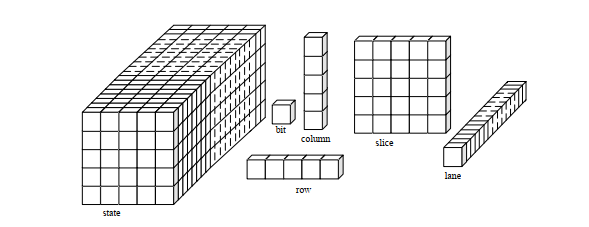
\includegraphics[width=0.7\linewidth]{constructure.PNG}  
		\caption{Terminologies used in Keccak}  
	\end{figure}
}

\frame{\frametitle{Analysis of the Keccak compression function}
	\begin{alertblock}{Keccak-$f[b]$ round function R}
		\begin{center}
			$R=\iota \circ \chi \circ \pi \circ \rho \circ \theta,$ with
		\end{center}

	\begin{itemize}
		\item $\theta : \quad a[x][y][z] \quad \leftarrow a[x][y][z]+\sum_{y^{\prime}=0}^{4} a[x-1]\left[y^{\prime}\right][z]+\sum_{y^{\prime}=0}^{4} a[x+1]\left[y^{\prime}\right][z-1]$
		
		\item $\rho : \quad a[x][y][z] \quad \leftarrow a[x][y][z-(t+1)(t+2) / 2], \  \text{with} \ t$ satisfying $0 \le t < 24$ \\ \qquad \qquad \qquad \quad  and $\left( \begin{array}{ll}{0} & {1} \\ {2} & {3}\end{array}\right)^{t} \left( \begin{array}{l}{1} \\ {0}\end{array}\right)=\left( \begin{array}{l}{x} \\ {y}\end{array}\right)$ in $G F(5)^{2 \times 2}$ or $t=-1$ \\ \qquad \qquad \qquad \quad if $x=y=0$
		
		\item $\pi : \quad \ a[x][y] \quad \ \ \leftarrow a\left[x^{\prime}\right]\left[y^{\prime}\right],$ with $\left( \begin{array}{l}{x} \\ {y}\end{array}\right)=\left( \begin{array}{ll}{0} & {1} \\ {2} & {3}\end{array}\right) \left( \begin{array}{l}{x^{\prime}} \\ {y^{\prime}}\end{array}\right)$
		
		\item $\chi : \quad \ \  a[x] \qquad \ \leftarrow a[x]+(a[x+1]+1) a[x+2]$
		
		\item $\iota \ : \quad \quad \ a \quad \quad \ \ \leftarrow a+R C\left[i_{r}\right]$
	\end{itemize}
	        	    
	\end{alertblock}	
}

\frame{\frametitle{Analysis of the Keccak compression function, cont.}
	\begin{alertblock}{Keccak-$f[b]$ round function R}
		
		\begin{itemize}
			\item $\theta : \quad \ \ {\color{blue}{Linear}} \quad \  \operatorname{deg}(\theta(x)) \leq \operatorname{deg}(x)$
		\end{itemize}
		
	\end{alertblock}

	\begin{figure}[h]
	\centering  
	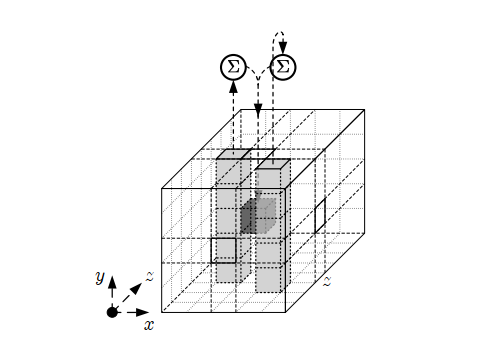
\includegraphics[width=0.7\linewidth]{theta.PNG}  
	\caption{$\theta$ applied to a single bit }    
	\end{figure}	
}

\frame{\frametitle{Analysis of the Keccak compression function, cont.}
	\begin{alertblock}{Keccak-$f[b]$ round function R}
		
		\begin{itemize}
		
			\item $\rho : \ {\color{blue}{Permutation}} \ \operatorname{deg}(\rho(x))=\operatorname{deg}(x)$
			
		\end{itemize}
		
	\end{alertblock}	

	\begin{figure}[h]
		\centering  
		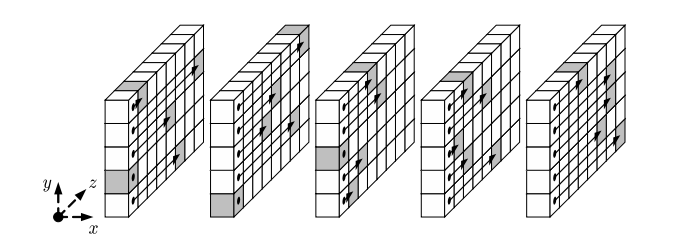
\includegraphics[width=0.7\linewidth]{rho.PNG}  
		\caption{$\rho$ applied to a slice }    
	\end{figure}
	
}

\frame{\frametitle{Analysis of the Keccak compression function, cont.}
	\begin{alertblock}{Keccak-$f[b]$ round function R}
		
		\begin{itemize}
					
			\item $\pi : \ {\color{blue}{Permutation}} \ \operatorname{deg}(\pi(x))=\operatorname{deg}(x)$	
		\end{itemize}
	\end{alertblock}

	\begin{figure}[h]
		\centering  
		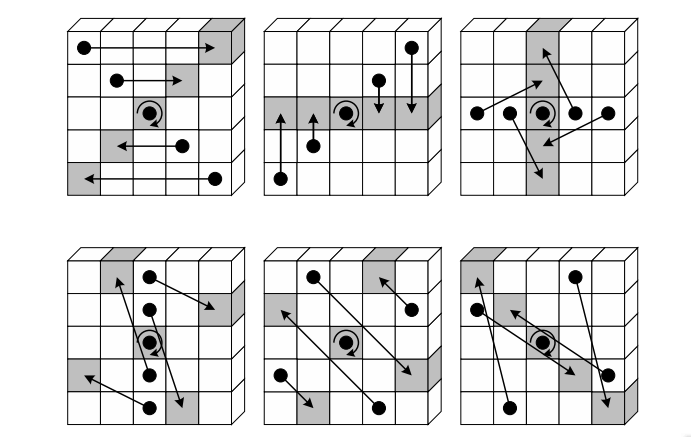
\includegraphics[width=0.7\linewidth]{pi.PNG}  
		\caption{$\pi$ applied to a slice }    
	\end{figure}	
}

\frame{\frametitle{Analysis of the Keccak compression function, cont.}
	\begin{alertblock}{Keccak-$f[b]$ round function R}
			
		\begin{itemize}
			
			\item $\chi : \ $ {\color{blue}{Non-linear}}   $ \ \operatorname{deg}(\chi(x)) \leq 2 \cdot \operatorname{deg}(x)$
			
		\end{itemize}
		
	\end{alertblock}
	
	\begin{figure}[h]
		\centering  
		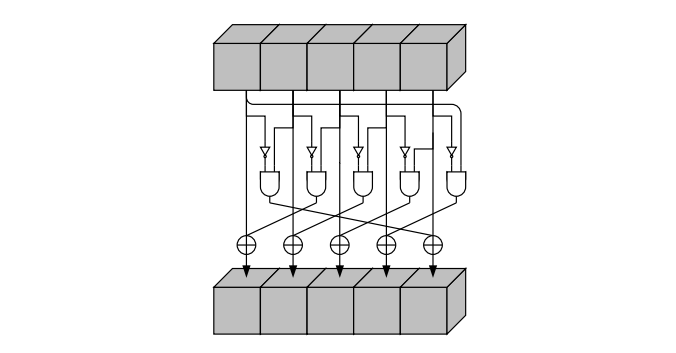
\includegraphics[width=0.7\linewidth]{chi.PNG}  
		\caption{$\chi$ applied to a sigle row }    
	\end{figure}	
}

\frame{\frametitle{Analysis of the Keccak compression function, cont.}
	\begin{alertblock}{Keccak-$f[b]$ round function R}
		\begin{center}
			$R=\iota \circ \chi \circ \pi \circ \rho \circ \theta,$ with
		\end{center}
		
		\begin{itemize}
			\item $\theta : \quad \ \ Linear \quad \  \operatorname{deg}(\theta(x)) \leq \operatorname{deg}(x)$
			
			\item $\rho : \ Permutation \ \operatorname{deg}(\rho(x))=\operatorname{deg}(x)$
			
			\item $\rho : \ Permutation \ \operatorname{deg}(\pi(x))=\operatorname{deg}(x)$
			
			\item $\chi : \  \ $ Non-linear   $  \operatorname{deg}(\chi(x)) \leq 2 \cdot \operatorname{deg}(x)$
			
			\item $\iota \ : \quad \ \ {\color{blue}{Linear}} \quad   \operatorname{deg}(\iota(x)) \leq \operatorname{deg}(x)$
		\end{itemize}
		
	\end{alertblock}

	\begin{center}
		So the degree of Keccak-$f[b]$ at most {\color{blue}{double}} with each round.
	\end{center}	
}

\frame{\frametitle{keyed modes of Keccak}
\begin{itemize}
	\item \textbf{MAC based on Keccak} A message authentication code (MAC) is used for verifying data integrity and authentication of a message. A secure MAC is expected to satisfy two main security properties.Assuming that an adversary has access to many valid message-tag pairs:
	\begin{itemize}
		\item it should be infeasible to recover the secret key used 
		\item it should be infeasible for the adversary to forge a MAC namely, provide a valid message-tag pair $ (M,T) $ for a message $M$ that has not been previously authenticated.
	\end{itemize}
\end{itemize}
	\begin{figure}[h]
		\centering  
		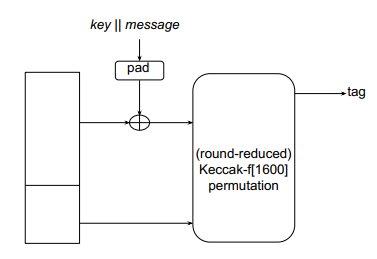
\includegraphics[width=0.5\linewidth]{mac.png}  
		\caption{MAC based on Keccak}  
		\label{fig:MAC based on Keccak}   
	\end{figure}
	
	
}

\frame{\frametitle{keyed modes of Keccak, cont.}
	\begin{itemize}
		\item \textbf{stream cipher based on Keccak} In the stram cipher mode, the state is initialized with the secret key, concatenated with a public initialization vector (IV). After each Keccak permutation call, an $r$-bit keystream (where $r$ is the bitrate of the Keccak instance) is extracted and used to encrypt a plaintext via bitwise XOR. In this paper, we only exploit the first $r$ bits of keystream, such that the internal permutation is applied only once.
	\end{itemize}
	\begin{figure}[h]
		\centering  
		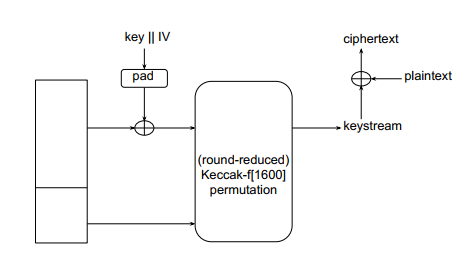
\includegraphics[width=0.5\linewidth]{streamcipher.png}  
		\caption{stram cipher based on Keccak}  
		\label{fig:stram cipher based on Keccak}   
	\end{figure}
	
	
}

\frame{\frametitle{key recovery attack on 5-round Keccak working as MAC}
	
	We attack the default variant of Keccak with a 1600-bit state (r=1024,c=576), where the number of rounds of the internal permutation is reduced to 5. The key and tag sizes are both 128 bit.
	\begin{itemize}
		\item \textbf{Preprocessing Phase} To find useful cubes for our attack, we randomly pick 31 out of the 128 public variable and check whether the superpoly consists of any secret variable or it is a constant. With the simple strate-\\gy, we have been able to find 117 linearly independent expressions in a few days, but as only 20-25\% of the superpolys are useful.
		
		\item \textbf{Online Phase} The attacker computes the actual binary value of a given superpoly by summing over the outputs obtained from the corresponding cube. There are 19 cubes used in this attack, each cube with 31 variab-\\les. Thus, the attacker obtains $19\cdot2^{31} \cong 2^{35}$ outputs for the 5-round Keccak.
	\end{itemize}
}

\frame{\frametitle{key recovery attack on 6-round Keccak working in stream cipher mode}
	\begin{itemize}
		\item A direct extension of the attack to 6 rounds seems infeasible as we would deal with polynomials of approximate degree $2^6=64$ and it is very unlikely to find (in reasonable time) cubes with linear superpolys.
		
		\item However, one more round can be reached by exploiting a specific property of  the Keccak $\chi$ step. As $\chi$ operates on the rows independent, if a whole row (5 bits) is known, we can invert these bits through $\iota$ and $\chi$ from given output bits. Consequently, the final nonlinear step $\chi$ can be inverted and the cube attack is reduced to 5.5 round.
	\end{itemize}

	\begin{table}
		\centering
		\caption{Boolean components of $\chi$ and $\chi^{-1}$ }
		\scriptsize
		\begin{tabular}{|c|c|c|c|}
			\hline
			
			Output    &  Corresponding Boolean function  &	Output    &  Corresponding Boolean function    \\ \hline
			$\chi_{0}$    & $x_{0}+x_{2}+x_{1} x_{2}$     & $\chi_{0}^{-1}$    & $x_{0}+x_{2}+x_{4}+x_{1} x_{2}+x_{1} x_{4}+x_{3} x_{4}+x_{1} x_{3} x_{4}$    \\ \hline
		
			$\chi_{1}$    & $x_{1}+x_{3}+x_{2} x_{3}$     &  	$\chi_{1}^{-1}$    & $x_{0}+x_{1}+x_{3}+x_{0} x_{2}+x_{0} x_{4}+x_{2} x_{3}+x_{0} x_{2} x_{4}$  \\ \hline
			
			$\chi_{2}$    & $x_{2}+x_{4}+x_{3} x_{4}$   & 	$\chi_{2}^{-1}$    & $x_{1}+x_{2}+x_{4}+x_{0} x_{1}+x_{1} x_{3}+x_{3} x_{4}+x_{0} x_{1} x_{3}$  \\ \hline
			
			$\chi_{3}$    & $x_{0}+x_{3}+x_{0} x_{4}$    &  $\chi_{3}^{-1}$    & $x_{0}+x_{2}+x_{3}+x_{0} x_{4}+x_{1} x_{2}+x_{2} x_{4}+x_{1} x_{2} x_{4}$   \\ \hline
			
			$\chi_{4}$    & $x_{1}+x_{4}+x_{0} x_{1}$    & 	$\chi_{4}^{-1}$    & $x_{1}+x_{3}+x_{4}+x_{0} x_{1}+x_{0} x_{3}+x_{2} x_{3}+x_{0} x_{2} x_{3}$     \\ \hline
		\end{tabular}
	\end{table}	

}

\frame{\frametitle{practical cube tester for 6.5-round Keccak permutation}
	
	We show how to  construct a practical cube tester for the 6.5-round Keccak permutation. As the expected algebraic degree for 6-round Keccak is 64, such an attack may seem at first impractical. However, if we carefully choose the cube variables, we can exploit a special property of $\theta$ in order to considerably reduce the output degree after 6 rounds and keep the complexity low.
	\begin{itemize}
		\item The well-known property of $\theta$ is that its action depends on the \textbf{column parities} only. Thus, if we set the cube variables in such a way that all the column parties are constants for all the possible variable values, then $\theta$ will not diffuse these variables throughout the state.
		\item Moreover, as $\rho$ and $\pi$ only permute he bits of the state, it is easy to choose the cube variables such that after the linear part of the round, they are not multiplied with each other through the subsequent non-linear $\chi$ layer. Consequently, the algebraic  degree of the state bits in the cube variables remains 1 after the first round, and it is at most 32 after 6 rounds.
	\end{itemize}

	
}


\frame{\frametitle{practical cube tester for 6.5-round Keccak permutation, cont.}
	

	\begin{itemize}
		\item We choose the 33-dimensiional cube $\left\{v_{0}, v_{1}, \ldots, v_{32}\right\}$ such that $v_{i}=A[0,2, i]$, while ensuring that the column parities remain constant by setting the additional linear constraints $A[0,3, i]= v_{i} \oplus c_{i}$, for arbitrary binary constants $c_{i}$. In other words, we sum over the outputs of the 33-dimensional linear subspace defined on the 66 state bits $A[0,2, i], A[0,3, i]$ by 33 equations $A[0,2, i]=A[0,3, i] \oplus c_{i}$ for $i \in\{0,1, \ldots, 32\}$. The remaining bits of the iinput state are set to arbitrary constants. At teh input to $\chi$, each 5-bits row of the state contains at most one variable, and therefore, the variables are not multiplied together in the first round as required.
		
		\begin{figure}[h]
			\centering  
			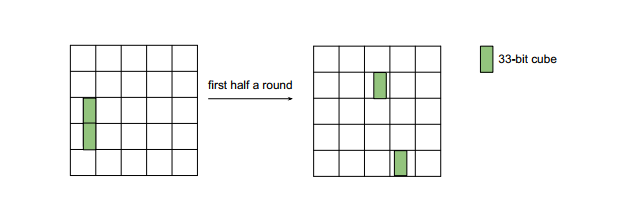
\includegraphics[width=0.5\linewidth]{initial_state.png}  
			\caption{The initial state of a cube tester and the transition through the first linear part of the round ($\theta$,$\rho$,
				$\pi$ steps)}  
			\label{fig:stram cipher based on Keccak}   
		\end{figure}
		
	\end{itemize}
	
	
}

\frame{\frametitle{practical cube tester for 6.5-round Keccak permutation, cont.}
	
	
	\begin{itemize}
		\item Since the degree of the output polynomials in the cube variable agter 6 rounds in only 32, the cube sum of any output bit after 6 rounds is equal to zero, which is a clear non-random property. Moreover, we can add a (linear) half-round and obtain a 6.5 round distinguisher using the same cube. If we assume that we can obtain sufficiently many output bits in order ot partially  invert the non-linear layer, we can extend the attack to 7 rounds in practical time.
		\item Assume that the 33-dimensional cube is missing an output for one value of the public variable. Then, as the sums of all $2^{33}$ output is zero, the missing output is equal to the sum of the remaining $2^{33}-1$ outputs. Thus, the distinguisher attack can be used to predict the output of the cipher for a previously unseen input value. 
	\end{itemize}
	
	
}


\frame{\frametitle{Divide-and-Conquer key recovery attack on Keccak-based MAC}
	
	
	\begin{itemize}
		\item As it is not clear how to use the standard key recovery techniques in our case, we use a different approach. The main idea in our attack is to select the public variables of the cube in such a way that the superpolys depend only on a (relatively) small number of key bits, whose value can be recovered independently of the rest of the key. Thus, the full key can be recovered in several phases in a divide-and-conquer manner.
		
		\item \textbf{Borderline Cubes} The starting point of the attack is the cube tester, which is based on a 33-variable cube, whose column parities remain constant for all of their $2^{33}$ possible values. As the cube variables are not multiplied together in the first round and the degree of 6-round Keccak in the state variables after one round is $2^5=32$, then the cube sums for the 33-variables are zero for all output bits. When we remove one variable from this cube, the sums are no longer guaranteed to be zero and they depend on the values of some of the constant bits of the state. This leaves us a borderline situation.
	\end{itemize}
	
	
}

\frame{\frametitle{Divide-and-Conquer key recovery attack on Keccak-based MAC, cont.}
	
	
	If a state bit is not multiplied with the cube variables in the first round, then the cube sums do not depend on the value of this bit. On the other hand, if a state bit is multiplied with the cube variables in the first round, then the cube sums generally depend on the value of the bit (assuming sufficient mixing of the state by the Keccak mapping). Thus, by a careful selection of a "borderline" cube of dimension 32, we can assure that the cube sums depend only on a (relatively) small number of key bits.
	
	
}

\frame{\frametitle{Divide-and -Conquer key recovery attack on Keccak-based MAC, cont.}
	
\textbf{Basic 6-round attack}
\begin{itemize}
	\item According to the Keccak MAC specification the 128-bit key is placed in $A[0,0]$ and $A[1,0]$. However, it is worth noting that our attack could be easily adapted to any other placements of the secret key. We select 32 cube variables $v_{1}, v_{2}, \dots, v_{32}$ in  $A[2,2]$ and $A[2,3]$, such that the column parities of  $A[2,*]$ remain constant for the $2^{32}$ possible values of the variables. This careful selection of the cube variables leads to two properties on which our attack is based:
	\begin{property}
		The cube sum of each output bit after 6 rounds does not depend on the value of $A[1,0]$.
	\end{property}

	\begin{property}
		The cube sum of each output bit after 6 rounds  depend on the value of $A[0,0]$.
	\end{property}
\end{itemize}	
	
}

\frame{\frametitle{Divide-and -Conquer key recovery attack on Keccak-based MAC, cont.}
	\begin{itemize}
		\item We now describe the attack which exploits the two properties to retrieve the value of $A[0,0]$. We separate the attack to preprocessing and online phase, where the preprocessing phase does not depend on the online values of the secret key. However, we take into account both of the phases when calculating the complexity of the full attack. 
		
		The preprocessing phase is described below.
		\begin{itemize}
			\item Set the capacity lanes $(A[1,4], A[2,4], A[3,4], A[4,4])$ to zero. Set all other state bits (beside $A[0,0]$ and the cube variables) to an arbitrary constant.
			\item For each of the $2^{64}$ possible values of $A[0,0]$: calculate the cube sums after 6 rounds for all the output bits. Store the cube sums in a sorted list $L$, next to the value of the corresponding $A[0,0]$.
		\end{itemize}
	
		The online phase, which is retrieves $A[0,0]$, is described below.
		\begin{itemize}
			\item Request the outputs for the $2^{32}$ messages that make up the chosen cube (using the same constant as in the preprocessing phase).
			
			\item Calculate the cube sums for the output bits and search them in $L$
			
			\item For each match in $L$, retrieve $A[0,0]$ and store all of its possible values.
			
		\end{itemize}
	\end{itemize}
		
	
}

\frame{\frametitle{Divide-and -Conquer key recovery attack on Keccak-based MAC, cont.}

	 Although the actual online value of $A[1,0]$ does not necessarity match its value used during preprocessing ,according to Property 1; it does not affect the cube sums. Thus, we will obtain a match with the correct value of $A[0,0]$. In order to recover $A[1,0]$, we independently apply a similar attack using 32 public variables in $A[4,2]$ and $A[4,3]$ (for which properties corresponding to Property 1 and Property 2 would apply). Finally, in order to recover the full key, we enumerate and test all combinations of the suggestions independently obtained for $A[0,0]$ and $A[1,0]$.
		
	
}


\section{Conditional cube attack on reduced-round \protect \\ Keccak sponge functon}

\frame {\frametitle{conditional cube tester for Keccak sponge function}
	
	\begin{figure}[h]
		\centering  
		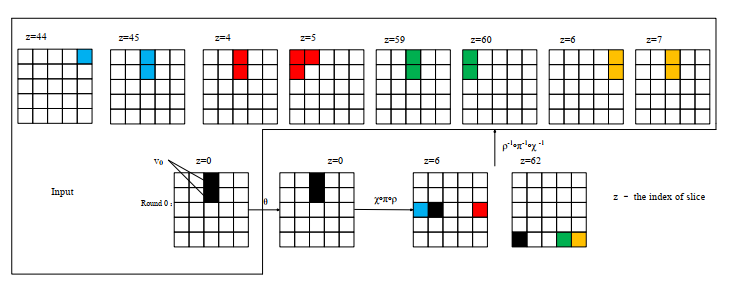
\includegraphics[width=0.8\linewidth]{bit-condition.PNG}  
		\caption{Overview of bit conditions}  
		\label{fig:bit condition.PNG}   
	\end{figure}
	
	The idea of our new model-the \textit{conditional cube tester}, is to attack some bit conditions to a cube tester.
}

\frame {\frametitle{conditional cube tester for Keccak sponge function}
	
	\begin{definition}
		Cube variables that have propagation controlled in the first round and are not multiplied with each other after the second round of Keccak are	called\textbf{ conditional cube variables}. Cube variables that are not multiplied with each other after the first round and are not multiplied with any conditional cube variable after the second round are called \textbf{ordinary cube variables}.
	\end{definition}
	
	
	\begin{theorem}
		For $(n+2)$-round Keccak sponge function  $(n>0)$, if there are $p \left(0 \leq p<2^{n}+1\right)$ conditional cube variables $v_{1}, \dots, v_{p}$, and $q=2^{n+1}-2p+1$, ordinary cube variables, $u_{1}, \ldots, u_{q}$ ( If $ q=0 $, we set $p=2^{n}+1$), then the term $v_{1} v_{2} \dots v_{p} u_{1} \dots u_{q}$ will not appear in the output polynomials of  $(n+2)$-round Keccak sponge function.
	\end{theorem}
	
}

\frame {\frametitle{Properties of Keccak sponge function}
	
	\begin{definition}
		Given a Boolean function $f\left(x_{0}, x_{1}, \dots, x_{n-1}\right)$, the bitwise derivative of $ f $ with respect to the variable $ x_{m} $ is defined as $$
		\delta_{x_{m}} f=f_{x_{m}=1}+f_{x_{m}=0}	$$
		The 0-th bitwise derivative is defined to be $ f $ itself. The i-th, where $ i \ge 2 $, bitwise
		derivative with respect to the variable sequence $\left(x_{m_{1}}, \dots, x_{m_{i}}\right)$ is defined as $$\delta_{x_{m_{1}}, \ldots, x_{m_{i}}}^{(i)} f=\delta_{x_{m_{i}}}\left(\delta_{x_{m_{1}}, \ldots, x_{m_{i-1}}}^{(i-1)} f\right)$$
	\end{definition}
}

\frame {\frametitle{Properties of Keccak sponge function}
	
	\begin{property}
		(\textbf{Bit Conditions}) IF $\delta_{v_{0}} F=(1,0,0,0,0)$, then $\delta_{v_{0}} G=(1,0,0,0,0)$ if and only if $f_{1}=0$ and $f_{4}+1=0$.
	\end{property}

	\begin{proof}
		By the structure of $\chi$, the algebraic representation of the output Boolean
		function $ G $ is given by the following equations:
		$$
		\begin{aligned} g_{0} &=f_{0}+\left(f_{1}+1\right) f_{2} \\ g_{1} &=f_{1}+\left(f_{2}+1\right) f_{3} \\ g_{2} &=f_{2}+\left(f_{3}+1\right) f_{4} \\ g_{3} &=f_{3}+\left(f_{4}+1\right) f_{0} \\ g_{4} &=f_{4}+\left(f_{0}+1\right) f_{1} \end{aligned}$$
	\end{proof}
}

\frame {\frametitle{Properties of Keccak sponge function, cont.}
	
	\begin{proof}
		From the definition of the bitwise derivative, it can be deduced that $\delta_{v_{0}} G=\left(1,0,0, f_{4}+1, f_{1}\right)$. It is clear that $\delta_{v_{0}} G=(1,0,0,0,0)$ if and only if $f_{1}=0$ and $f_{4}+1=0$.
	\end{proof}

	\begin{figure}
		\centering
		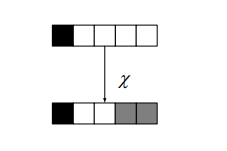
\includegraphics[width=0.5\linewidth]{Diffusion-caused-by-operation-chi}
		\caption{Diffusion caused byoperation $\chi$}
		\label{fig:diffusion-caused-by-operation-chi}
	\end{figure}
	
}

\frame {\frametitle{Properties of Keccak sponge function, cont.}
	
	\begin{figure}
		\centering
		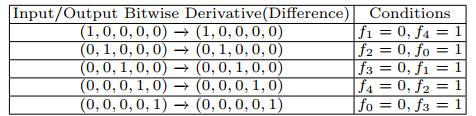
\includegraphics[width=0.7\linewidth]{confitions-for-bitwise-derivative}
		\caption{Summary of conidtions for bitwise derivative of $\chi$}
		\label{fig:confitions-for-bitwise-derivative}
	\end{figure}
	The input and output have the same vector of bitwise derivatives so that the propagation
	of $ v_{0} $ by $\chi$ is under control. This will be used in constructing our conditional cube tester.
	
}


\frame {\frametitle{Properties of Keccak sponge function, cont.}
	\begin{figure}
		\centering
		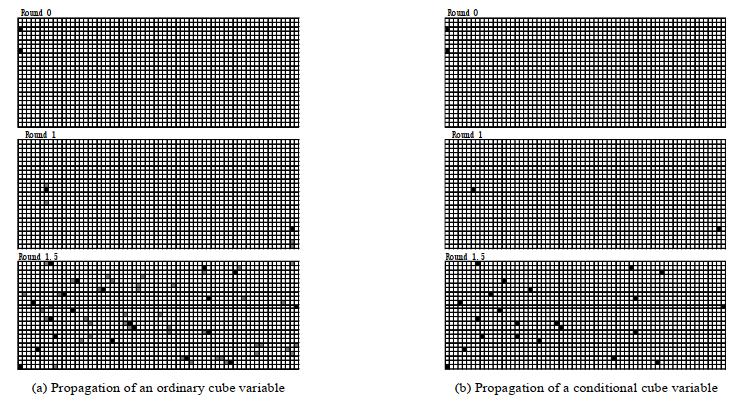
\includegraphics[width=0.7\linewidth]{a-conditional-cube-variable}
		\caption{1.5 round differential of an ordinary and a conditional cube variable}
		\label{fig:a-conditional-cube-variable}
	\end{figure}
	
	
}

\frame {\frametitle{Properties of Keccak sponge function, cont.}

	\begin{property}
		(\textbf{Multiplication}) Assume that $\delta_{v_{0}} F=\left(\delta_{v_{0}} f_{0}, 0,0,0,0\right)$ and $\delta_{v_{1}} F=\left(0, \delta_{v_{1}} f_{1}, 0,0,0\right)$ with $\delta_{v_{0}} f_{0} \cdot \delta_{v_{1}} f_{1} \neq 0$, then the term $ v_{0}v_{1} $ will be in the output of $\chi$.
	\end{property}	

	\begin{proof}
		The component $ g_{4} $ of the	output  $G=\left(g_{0}, g_{1}, g_{2}, g_{3}, g_{4}\right)$ is $f_{4}+\left(f_{0}+1\right) f_{1}$. From
		$$
		\delta_{v_{0}, v_{1}}^{(2)} g_{4}=\delta_{v_{1}}\left(\delta_{v_{0}} g_{4}\right)=\delta_{v_{1}}\left(\delta_{v_{0}} f_{0}\right) \cdot f_{1}+\delta_{v_{0}} f_{0} \cdot \delta_{v_{1}} f_{1}=\delta_{v_{0}} f_{0} \cdot \delta_{v_{1}} f_{1}$$
		
		we see that $\delta_{v_{0}, v_{1}}^{(2)} g_{4} \neq 0$ and hence $ g_{4} $ contains the term $ v_{0}v_{1} $. In particular, if $\delta_{v_{0}} f_{0}=\delta_{v_{1}} f_{1}=1,$ then $g_{4}=v_{0} v_{1}+h$, where $ h $ is a Boolean function not divisible	by $ v_{0}v_{1} $.
	\end{proof}
	
}

\frame {\frametitle{Properties of Keccak sponge function, cont.}
	
	\begin{property}
		(\textbf{Exclusion}) If $\delta_{v_{0}} F=(1,0,0,0,0)$ and $\delta_{v_{1}} F=(0,0,1,0,0)$, then at least one of $\delta_{v_{0}} G=(1,0,0,0,0)$ and $\delta_{v_{1}} G=(0,0,1,0,0)$ is false.
	\end{property}	
	
	\begin{proof}
		The conditions $\delta_{v_{0}} F= (1,0,0,0,0)$ and $\delta_{v_{0}} G=(1,0,0,0,0)$ would imply $f_{1}=0, f_{4}=1$. Under the assumption $\delta_{v_{1}} F=(0,0,1,0,0),$ if $\delta_{v_{1}} G=(0,0,1,0,0)$ also holds true, then we would have $f_{1}=1, f_{3}=0$.
	\end{proof}
	
}

\frame {\frametitle{General process for key recovery attack on Keccak-MAC}
	
	\begin{enumerate}[(1)]
		\item Assign free variables with random values.
		\item Guess values of the s equivalent key bits.
		\item Calculate the values of conditional variables under the guess of key bits.
		\item For each possible set of values of cube variables, compute the corresponding tag and then sum all of the 128-bit tags over the $\left(2^{n+1}-p+1\right)$-
		dimension cube.
		\item If the sum is zero, the guess of these s key bits is probable correct and
		the process terminates; otherwise the guess is invalid, go back to Step 2.
	\end{enumerate}
	
	Time Complexity:$\frac{1}{s} \cdot 2^{n+1}-p+s+8=\frac{2^{s-p}}{s} \cdot 2^{2^{n+1}+8}$
}

\frame {\frametitle{General process for key recovery attack on Keccak-MAC, cont.}
	\begin{figure}
		\centering
		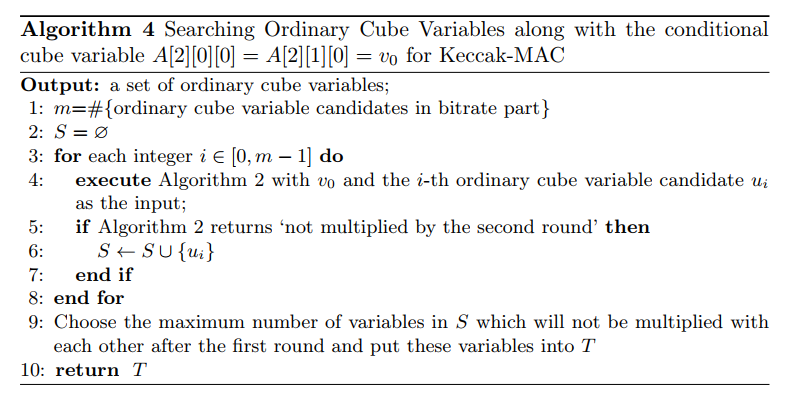
\includegraphics[width=0.7\linewidth]{algorithm4}
		\caption{Search ordinary cube variable}
		\label{fig:algorithm4}
	\end{figure}
	
}

\frame {\frametitle{key recovery on 5/6/7-round Keccak-MAC}

	conditional cube variable: $A[2][0][0]=A[2][1][0]=v_{0}$\\
	bit conditions: $\delta_{v_{0}} A[2][0][6]=
	\delta_{v_{0}} A[2][4][6]=\delta_{v_{0}} A[4][3][62]=\delta_{v_{0}} A[4][4][62]=0$ 
	\begin{figure}
		\centering
		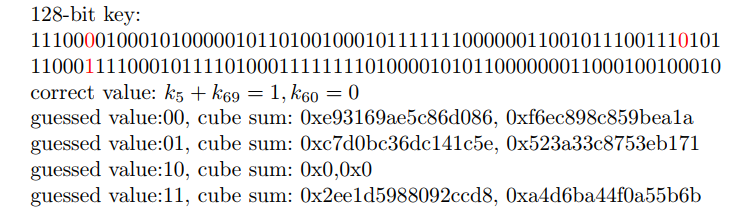
\includegraphics[width=1.0\linewidth]{correctkey}
		\caption{Distinguish the correct key}
		\label{fig:correctkey}
	\end{figure}
	
}

\frame {\frametitle{key recovery on 5/6/7-round Keccak-MAC, cont.}
	
	\begin{figure}
		\centering
		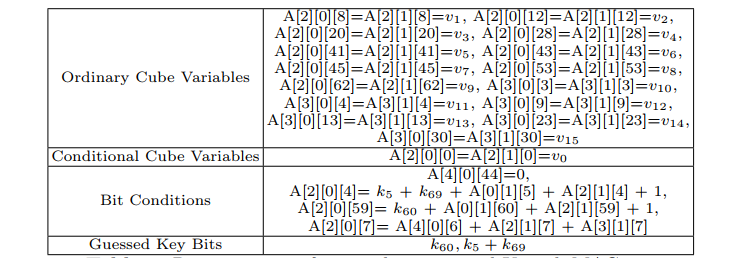
\includegraphics[width=1.0\linewidth]{bit-condition-parameters}
		\caption{Parameters set for attack on 5-round Keccak-MAC-512}
		\label{fig:bit-condition-parameters}
	\end{figure}
	
	
}

\frame {\frametitle{}
	~~~~~~~~~~~~~~~~~~~~~~~~~~~~~~~~~~~~Thank You For Your Attention!
}
\end{document}

